%------------------------------------------------------------------------------
% Beginning of journal.tex
%------------------------------------------------------------------------------
%
% AMS-LaTeX version 2 sample file for journals, based on amsart.cls.
%
%        ***     DO NOT USE THIS FILE AS A STARTER.      ***
%        ***  USE THE JOURNAL-SPECIFIC *.TEMPLATE FILE.  ***
%
% Replace amsart by the documentclass for the target journal, e.g., tran-l.
%
\documentclass{amsart}

%     If your article includes graphics, uncomment this command.
\usepackage{graphicx}

\newtheorem{theorem}{Theorem}[section]
\newtheorem{lemma}[theorem]{Lemma}

\theoremstyle{definition}
\newtheorem{definition}[theorem]{Definition}
\newtheorem{example}[theorem]{Example}
\newtheorem{xca}[theorem]{Exercise}

\theoremstyle{remark}
\newtheorem{remark}[theorem]{Remark}

\numberwithin{equation}{section}

%    Absolute value notation
\newcommand{\abs}[1]{\lvert#1\rvert}

%    Blank box placeholder for figures (to avoid requiring any
%    particular graphics capabilities for printing this document).
\newcommand{\blankbox}[2]{%
  \parbox{\columnwidth}{\centering
%    Set fboxsep to 0 so that the actual size of the box will match the
%    given measurements more closely.
    \setlength{\fboxsep}{0pt}%
    \fbox{\raisebox{0pt}[#2]{\hspace{#1}}}%
  }%
}

% user added
\usepackage{longtable}
\usepackage{dot2texi}
\usepackage{tikz}
\usetikzlibrary{automata,shapes,arrows}


\def\tr{\mathrm{tr}}
\def\Path{\mathrm{Path}}
\def\hier{\mathrm{Hier}}
\def\Vertex{\mathrm{Vertex}}
\def\adj{\mathrm{adj}}

\begin{document}

\title{Ensemble Stability of Biological Networks}

%    Information for first author
\author{Aviv Bergman}
%    Address of record for the research reported here
\address{Department of Systems and Computational Biology, Albert Einstein College of Medicine, Bronx, New York 10461}
%    Current address
\curraddr{}
\email{aviv@einstein.yu.edu}
%    \thanks will become a 1st page footnote.
% \thanks{The first author was supported in part by NSF Grant \#000000.}

%    Information for second author
\author{Raymond S. Puzio}
\address{Department of Systems and Computational Biology, Albert Einstein College of Medicine, Bronx, New York 10461}
%    Current address
\curraddr{}
\email{rsp@novres.org}
% \thanks{Support information for the second author.}

%    Information for third author
\author{Cameron Smith}
\address{Department of Systems and Computational Biology, Albert Einstein College of Medicine, Bronx, New York 10461}
%    Current address
\curraddr{}
\email{cameron.smith@med.einstein.yu.edu}
% \thanks{Support information for the second author.}

%    General info
% \subjclass[2000]{Primary 54C40, 14E20; Secondary 46E25, 20C20}

% \date{January 1, 2001 and, in revised form, June 22, 2001.}

% \dedicatory{This paper is dedicated to our advisors.}

% \keywords{Differential geometry, algebraic geometry}

\begin{abstract}
The analysis of dynamical systems that attempts to model chemical reaction, gene-regulatory, population, and ecosystem networks all rely on models having many parameters and thus many degrees of freedom. When the details of a system are unknown, one effective approach is to study the dynamical properties of a collection of models determined by constraints applying to all such systems. Here we analyze the stability of a large class of dynamical systems to perturbations in the underlying structure of the system: a property referred to as \emph{structural stability}. In particular, we precisely determine the probability distribution over system connectivity, a parameter which has significant implications from the study of gene-regulatory networks to ecosystem dynamics, of structural stability for systems with two and three interacting components. We show for these cases that structural stability has a non-monotonic relationship with system connectivity. We also demonstrate that networks with a hierarchical structure are more likely to be stable to perturbations than those with a more entangled heterarchical structure. These results support future work attempting to characterize the scaling relationship between structural stability and system connectivity. The latter investigation is necessary to evaluate several conjectured but ultimately untested hypotheses about biological networks.
\end{abstract}

\maketitle

\section{Introduction}

The traditional approach taken in the study of chemical reaction, gene-regulatory, population, and ecosystem networks is to consider a particular example, derive a system of differential equations to model that example, try to fit the model to data and adjust the modeling assumptions along with parameter values until a good fit is achieved. Recent work has demonstrated that as a result of sloppiness in the dependence of qualitative dynamic phenomena on the geometry of parameter space that this approach allows for a large variety of models to ``fit the data'' \cite{Brown2003,Gutenkunst2007,Daniels2008a,Machta2013,Hines2014,Prabakaran2014}. In the face of uncertainty about the structure of such biological networks, to model the components under consideration as randomly interlinked becomes a reasonable approximation. This approach enables one to gain insight into what dynamical phenomena are possible to observe within a given class of dynamical systems, which is necessary to understand in order to determine whether or not a particular dynamical phenomenon should be regarded as unique or generic in the development and investigation of models applied to particular systems \cite{Gunawardena2013,Gunawardena2014}.

Indeed, investigating generic properties of a large class of dynamical systems was the approach taken by May in models of ecosystem dynamics \cite{Gardner1970,May1972}. The class of dynamical systems studied by May is so general that to restrict its applicability to ecosystem dynamics is certainly not necessary and perhaps even inefficient with respect to the goal of understanding how biological networks operate across the various relevant levels of organization. For example, the study of chemical reaction, population, and gene-regulatory networks all utilize essentially equivalent mathematical structure as that discussed by May in the context of ecosystem dynamics \cite{RossCr2003,Alon2006,Palsson2006,HamidBolouri2008,Palsson2011a,Voit2012,Sauro2012}. Developing unified mathematical descriptions of all of these is one of the paramount goals of systems biology. This incredibly generic applicability of gaining a better understanding of the class of models investigated by May demonstrates the unequivocal value of deeper investigation.  However, work attempting to continue the development of the so-called May-Wigner stability theorem revealed that May's conjectured stability criterion was not as easy to demonstrate as was initially believed \cite{Cohen1984,May1972a,Radius2014}.

Here we build on work aimed at investigating the stability of randomly connected dynamical systems to state-based perturbations. We precisely compute the probability of stability as a distribution over system connectivity for all systems containing two interacting components. We then proceed to determine the probability of structural stability over the same domain. We find that while stability to perturbations in the state of this class of dynamical systems is independent of system connectivity, perturbations to the magnitude of connections is correlated with connectivity in a non-linear manner. This work reestablishes and clarifies a thread of research that is extremely important for the continuing development of systems biology.

\section{Stability analysis of biological networks}

Consider an n-dimensional vector
$$
x(t) = (x_1(t), \ldots x_n(t)) = \vec{x}(t)
$$
whose components are solutions to the arbitrary first order system
$$
\frac{dx_i(t)}{dt} = F_i(\vec{x}(t)), \; (i=1,\ldots,n)
$$
where $F_i$ represent, potentially nonlinear, functions of the given vector of state variables. We can associate a directed graph $G_X$ that describes the manner in which each of the variables depends upon one another given by an adjacency matrix $\adj(G_X)$ where
 \begin{displaymath}
   \adj(G_X)_{ij} = \left\{
     \begin{array}{ll}
       1, & F_i \hbox{ depends on } x_j\\
       0, & F_i \hbox{ does not depend on } x_j
     \end{array}
   \right.
\end{displaymath}
For example, given the system $X = \{\{x_1,x_2\},\{F_1,F_2\}\}$
\begin{align*}
\frac{dx_1}{dt} & = F_1(x_2)\\
\frac{dx_2}{dt} & = F_2(x_1,x_2)
\end{align*}
we have the graph
\begin{center}
\begin{tikzpicture}[
every state/.style={draw=red!50,very thick,fill=red!20}]
\begin{dot2tex}[styleonly,codeonly,neato,mathmode]
digraph G {
d2ttikzedgelabels = true;
node [style="state"];
edge [lblstyle="auto",topath="bend left",style="line width=1.5pt"];
x_1 -> x_2;
x_2 -> x_1;
x_2 -> x_2 [topath="loop above"];
}
\end{dot2tex}
\end{tikzpicture}
\end{center}
with adjacency matrix
$$
\adj(G_X) = \begin{pmatrix}
0 & 1 \\
1 & 1
\end{pmatrix}
$$

Linearization of the $F_i$ about any equilibrium solution $\vec{x}^0$ such that $F_i(\vec{x}^0)=0$ leads to the system
\begin{equation}\label{eq:lineardynsys}
\frac{d\vec{y}(t)}{dt} = A \vec{y}(t),
\end{equation}
where $\vec{y} = \vec{x} - \vec{x}^0$ and the $n \times n$-matrix $A$ has components
$$
a_{ij} = \left. \frac{\partial F_i}{\partial x_j} \right|_{\vec{x} = \vec{x}^0}.
$$
To each dynamical system having Jacobian matrix $A$ at some fixed point $\vec{x}^0$ we can associate a directed graph $G_A$ given by an adjacency matrix $\adj(G_A)$ where
 \begin{displaymath}
   \adj(G_A)_{ij} = \left\{
     \begin{array}{lr}
       1, & a_{ij} \neq 0\\
       0, & a_{ij} = 0
     \end{array}
   \right.
\end{displaymath}
The graphs $G_X$ and $G_A$ are equivalent because the condition $F_i$ independent of $x_j$ definitive of $\adj(G_X)$ corresponds precisely to $\frac{\partial F_i}{\partial x_j}=0$.

The spectral abscissa of the matrix $A$ is defined as
$$
\eta(A) = \max_i \{\Re(\lambda_i)\}
$$
where $\lambda_i$ are the eigenvalues of $A$. The system defined by $F_i$ and $\vec{x}^0$ is dynamically stable if the spectral abscissa of $A$ is less than zero, equivalently, $\eta(A) < 0$. This is because the general solution to equation \ref{eq:lineardynsys} is
$$
y_i(t) = \sum_j b_{ij} e^{\lambda_j t}, \; (i=1,\ldots,n)
$$
for some matrix $B=(b_{ij})$ and thus all $\vec{y} = \vec{x} - \vec{x}^0$ decay to zero when all $\lambda_i < 0$.

To determine whether a randomly selected dynamical system evaluated at a random critical point, given by a matrix such as $A$, is stable, it is sufficient to check the above condition. Integrating over the region of the parameter space defining $A$ enables the determination of the probability of stability to perturbations in state $\vec{x}$ over an ensemble of dynamical systems.

Another form of stability, referred to as structural stability \cite{Smale1967}, requires the determination of whether or not a given dynamical system that is determined to be stable remains stable under a perturbation to one of its defining parameters. This can be formalized as the conditional probability distribution
$$
P(A' \, \textrm{stable}\, \big| \, A \, \textrm{stable})
$$
where $A'$ represents a matrix derived from some perturbation applied to the matrix $A$ given above. In the simple case where $A \in \mathbb{R}^{n \times n}$ the perturbation which involves sampling uniformly over the $a_{ij}$ defining $A$ the value of a particular $a_{ij}$ from a given probability distribution.

\section{System graph and decomposition into strongly connected components}
We will show how the stability of the dynamical system associated to Jacobian $A$ is characterized by properties of the associated graph $G_A$. The characteristic polynomial $\chi(A)$ associated to $A$ can be factored according to the strongly connected components of the graph $G$. $${\chi(M)'(z) \over \chi(M)(z)} = \tr (zI - M)^{-1}$$ where, $\chi(M)(z) = \det (zI - M)$ is the chararacteristic polynomial of the matrix $M$ with $z$ a complex variable.  This formula is readily verified when $M$ is diagonal and has the nice property of being additive over decompositions of the matrix. Making the change of variables $x=\frac{1}{z}$, we have $$\tr (I - xM)^n = \sum_{n=0}^\infty x^n \sum_{a \in \Vertex(G)} \sum_{p \in \Path_n (G)(a,a)} F(p)$$
where $G$ is the graph of the matrix and $\Path_n (G;a,b)$ is the set of
paths of length $n$ from $a$ to $b$.  $(\Vertex(G), \Path(G), \cdot)$ is a category; $F$ is the functor from this category to the multiplicative semigroup of the real numbers which corresponds to the matrix $M$.

We now make use of the additivity.  Let $\hier$ be the functor which
sends $G$ to a poset $P$.  Then every element $p$ of $\Path(a,a)$ lies
in $\hier^{-1} (\hier(a))$.  Hence, our sum decomposes into partial sums
for the fibers of the points in the hierarchy which corresponds to a
factorization of the characteristic polynomial.


\section{Stability criteria}
We call a matrix $M$ stable if all its eigenvalues have negative real
part.  Define the polynomial $p(x) = \det(xI + M)$.  Then, since the
roots of $p$ are minus the eigenvalues of $M$, asking that $M$ be
stable is equivalent to asking that the roots of $p$ all have real
part.  We will formulate conditions for this to happen in terms of the coefficients of $p$.

Let us start by fixing some notation.  Suppose that $M$ is of size $n
\times n$.  Denote the coefficients of $p$ as $s_j$ and its roots as
$r_j$, writing $p(x) = x^n + \sum_{k=1}^n s_k x^{n-k} = \prod_{k=1}^n
(x-r_k)$.

Introduce $V$ as the parameter space of all polynomials of degree $n$
with real coefficients.  In other words, $V$ is a real vector space of
dimension $n$ whose coordinates we will identify with the coefficients
$s_k$ of our polynomial.  We now partition this space into regions
corresponding to specific types of polynomials.  Let $R_{abcd}$ be the
subset of $V$ such that $x \in R_{abcd}$ if and only if the polynomial
corresponding to $x$ has $a$ positive real roots, $b$ negative real
roots, $c$ complex roots with positive real part and $d$ complex roots
with negative real part.  Once we characterize these regions using
invariants, we will have solved the original problem because a matrix
is stable if the point of $V$ corresponding to it lies in a region of
the form $R_{a0c0}$.

Next, we introduce some products:
\begin{align}
D &= \prod_{k=1}^n r_n \cr
\delta &= \prod_{j=1}^{n-1} \prod_{k=j+1}^n (r_1 - r_j)^2 \cr
\Delta &= \prod_{j=1}^{n-1} \prod_{k=j+1}^n (r_1 + r_j) \cr
\end{align}

Since these quantities are invariant under permutation of the roots
$r_j$, they may be expressed as functions of the coefficients $s_j$.
The explicit expressions may be obtained by such techniques as long
division and determinants. These quantities are of interest because they describe the boundaries between the regions introduced above.

The simplest case is $n=2$.  There we have the regions $R_{2000},
R_{1100}, R_{0200}, R_{0020}, R_{0002}$ and our invariants are $D =
s_2, \delta = s_1^2 - 4s_2, \Delta = s_1$.  The relation between these
is summarized by the conditions
\begin{align}
R_{2000} \qquad &D > 0, \delta > 0, \Delta > 0, \cr
R_{1100} \qquad &D < 0, \delta > 0, \cr
R_{0200} \qquad &D > 0, \delta > 0, \Delta < 0, \cr
R_{0020} \qquad &\delta < 0, \Delta > 0, \cr
R_{0002} \qquad &\delta < 0, \Delta < 0. \cr
\end{align}
These regions used for the classification of stability of two-component systems are show in Fig. \ref{fig:region2x2}. The stable regions are given by $R_{2000}$ and $R_{0020}$. All of the other regions represent unstable matrices.

\begin{figure}[!ht]
\centering
\noindent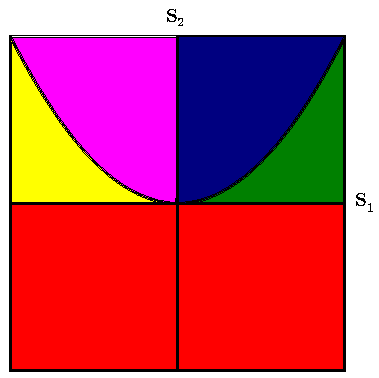
\includegraphics[width=0.5\columnwidth]{fig/region2x2.pdf}
\caption{{\bf Stability conditions on coefficients of the characteristic polynomial for two component systems.} The regions correspond to all possible relationships between the invariants determined by the characteristic polynomial. Colors correspond to the regions given in the main text Green: $R_{2000}$, Red: $R_{1100}$, Yellow: $R_{0200}$, Magenta: $R_{0002}$, Blue: $R_{0020}$.}
\label{fig:region2x2}
\end{figure}

Moving to $n=3$, our invariants now look as follows: $D = s_3, \delta
= 18 s_1 s_2 s_2 + s_1^2 s_2^2 - 4 s_2^3 - 4 s_1^3 s_3 - 27 s_3,
\Delta = s_1 s_2 - s_3$.  However, now we can no longer simply use their
signs to distinguish regions.  For instance, consider the regions
$R_{3000}$ and $R_{1200}$.  These both have $D > 0$ and $\delta > 0$
but to tell them apart, we need to note that the region $\delta > 0$
has two connected components and use the auxiliary condition that $s_1 > 0$ to
specify which of the components contains our region. The regions analogous to Fig. \ref{fig:region2x2} for three component systems where $D=1$ is given in Fig. \ref{fig:region3x3}.
%(Looking at the sign of $\Delta$ will not help here because, while $\Delta > 0$ in the region $R_{3000}$, it is also positive for some elements of $R_{1200}$ as well.)

\begin{figure}[!ht]
\centering
\noindent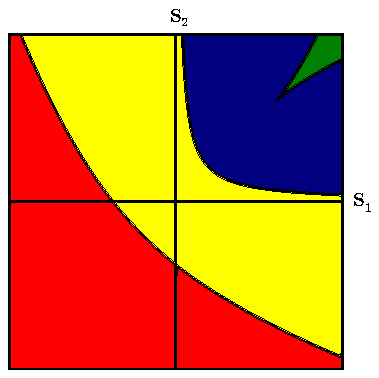
\includegraphics[width=0.5\columnwidth]{fig/region3x3.pdf}
\caption{{\bf Stability conditions on coefficients of the characteristic polynomial for three component systems.} Colors correspond to the following regions Green: $R_{3000}$, Red: $R_{1200}$, Yellow: $R_{1002}$, Blue: $R_{1020}$. This is the plane $s_3=1$.}
\label{fig:region3x3}
\end{figure}

\section{Two component systems}
For two-component systems having $2 \times 2$ Jacobian matrices, the aforementioned stability criteria result in the conditions $T < 0$ and $D >
0$ where $T$ and $D$ denote the trace and the determinant.

Suppose we have a stable matrix
$$
\begin{pmatrix}
a & b \\
d & c
\end{pmatrix}
$$
where $a + c < 0$ and $ac > bd$. We will consider the case in which each of the parameters defining the matrix is sampled from the uniform distribution $\mathcal{U}(-1,1)$ so that the parameter space corresponds to the $d$-dimensional hypercube, $H^d$, of edge length $r=2$, centered about the origin, and having volume $r^d$.  We want to know the probability that, if we resample an element of this matrix, the result will be stable.  By symmetry, there are two cases to consider; resampling $a$ is equivalent to resampling $c$ and resampling $b$ is equivalent
to resampling $d$.

Suppose that we resample $b$.  We want to compute the probability that a random stable matrix will remain stable upon resampling $b$, which is
% \begin{strip}
\begin{align}\label{eq:condprob}
P\left(\begin{pmatrix}
a & b' \\
d & c
\end{pmatrix} \textrm{stable } \bigg| \begin{pmatrix}
a & b \\
d & c
\end{pmatrix} \textrm{stable } \right)
& = \frac{P\left(\begin{pmatrix}
a & b \\
d & c
\end{pmatrix} \textrm{stable and } \begin{pmatrix}
a & b' \\
d & c
\end{pmatrix} \textrm{stable } \right)}{P\left(\begin{pmatrix}
a & b \\
d & c
\end{pmatrix} \textrm{stable } \right)}.
\end{align}
The denominator of \ref{eq:condprob} is given by
\begin{align*}
P\left(\begin{pmatrix}
a & b \\
d & c
\end{pmatrix} \textrm{stable } \right) = \frac{\int_{{ac>bd \atop a+c<0} \atop H^4} da\,db\,dc\,dd\,1}{\int_{H^4} da\,db\,dc\,dd\,1}.
\end{align*}
Since the trace does not involve $b$, the $T<0$ condition will be satisfied automatically and we only need to examine the determinant. Thus, we have the inequalities $ac > b'd$ and $-1 < b' < 1$ in addition to the previous constraints leading to an expression for the numerator of \ref{eq:condprob}
\begin{align*}
P\left(\begin{pmatrix}
a & b \\
d & c
\end{pmatrix} \textrm{stable and } \begin{pmatrix}
a & b' \\
d & c
\end{pmatrix} \textrm{stable } \right) = \frac{\int_{{{ac>b'd \atop ac>bd} \atop a+c<0} \atop H^5} da\,db\,dc\,dd\,db'\,1}{\int_{H^5} da\,db\,dc\,dd\,db'\,1}.
\end{align*}
The analogous equation for resampling $a$ is
\begin{align*}
P\left(\begin{pmatrix}
a & b \\
d & c
\end{pmatrix} \textrm{stable and } \begin{pmatrix}
a' & b \\
d & c
\end{pmatrix} \textrm{stable } \right) = \frac{\int_{{{{a'c>bd \atop a' + c < 0} \atop ac>bd} \atop a+c<0} \atop H^5} da\,db\,dc\,dd\,da'\,1}{\int_{H^5} da\,db\,dc\,dd\,da'\,1}.
\end{align*}

\newcommand{\specialcell}[2][c]{%
  \begin{tabular}[#1]{@{}c@{}}#2\end{tabular}}

\begin{table}[h]
\begin{tabular}{ c || c | c | c }
\hline
matrix & connectivity & \specialcell{probability of stability\\to perturbation} & probability of stability\\
\hline
  $\begin{pmatrix}
a & b \\
d & c
\end{pmatrix}$ & 4 & 0.62 & 0.25 \\
  $\begin{pmatrix}
a & b \\
d & 0
\end{pmatrix}$, $\begin{pmatrix}
0 & b \\
d & c
\end{pmatrix}$ & 3 & 0.5 & 0.25 \\
  $\begin{pmatrix}
a & 0 \\
d & c
\end{pmatrix}$, $\begin{pmatrix}
a & b \\
0 & c
\end{pmatrix}$ & 3 & 0.67 & 0.25 \\
$\begin{pmatrix}
a & 0 \\
0 & c
\end{pmatrix}$ & 2 & 0.5 & 0.25 \\
\end{tabular}
\caption{{\bf Probability of stability under resampling and \emph{a priori} stability for two component systems derived analytically}. All matrices not listed have $0$ probability of stability.}\label{tab:structstabmat}
\end{table}

The probability of \emph{a priori} stability and of stability to perturbations for all two component systems is given in Table \ref{tab:structstabmat}.

\section{Three component systems}

The probability of \emph{a priori} stability and of stability to perturbations for all three component systems is given in Table \ref{tab:structstabmat3}. Fig. \ref{fig:connectcycle3D3x3} shows the probability of stability to perturbations for all three component systems as a function of connectivity and number of cycles. Fig. \ref{fig:stab3x3} shows the probability of stability to perturbations for all three component systems as a function of connectivity. Fig. \ref{fig:cycle3x3} shows the probability of stability to perturbations for all three component systems as a function of the number of simple cycles (elementary circuits) of length greater than one in the corresponding directed graph \cite{Johnson1975}.

\begin{figure}[!ht]
\centering
\noindent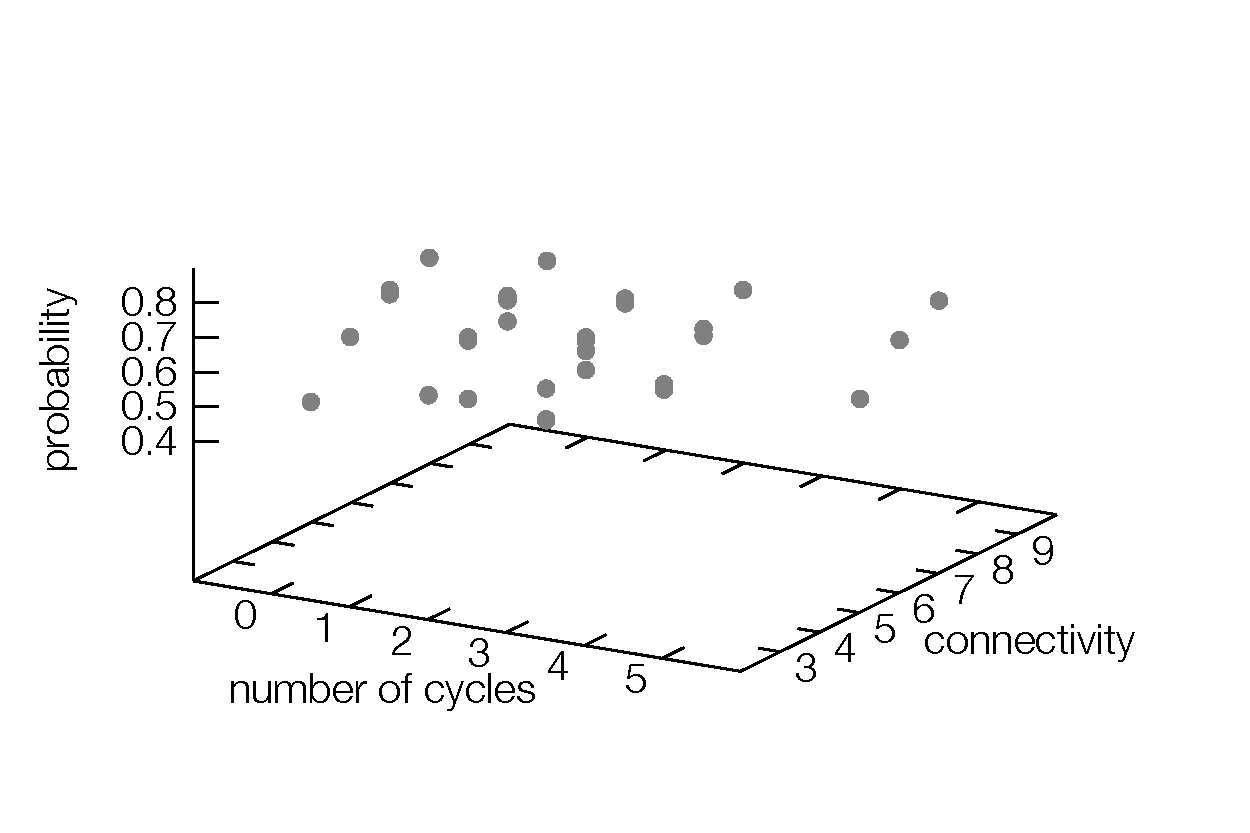
\includegraphics[width=0.8\columnwidth]{fig/connectcycle3D3x3.pdf}
\caption{{\bf Plot of stability to perturbations versus number of cycles and connectivity for three component systems.} }
\label{fig:connectcycle3D3x3}
\end{figure}

\begin{figure}[!ht]
\centering
\noindent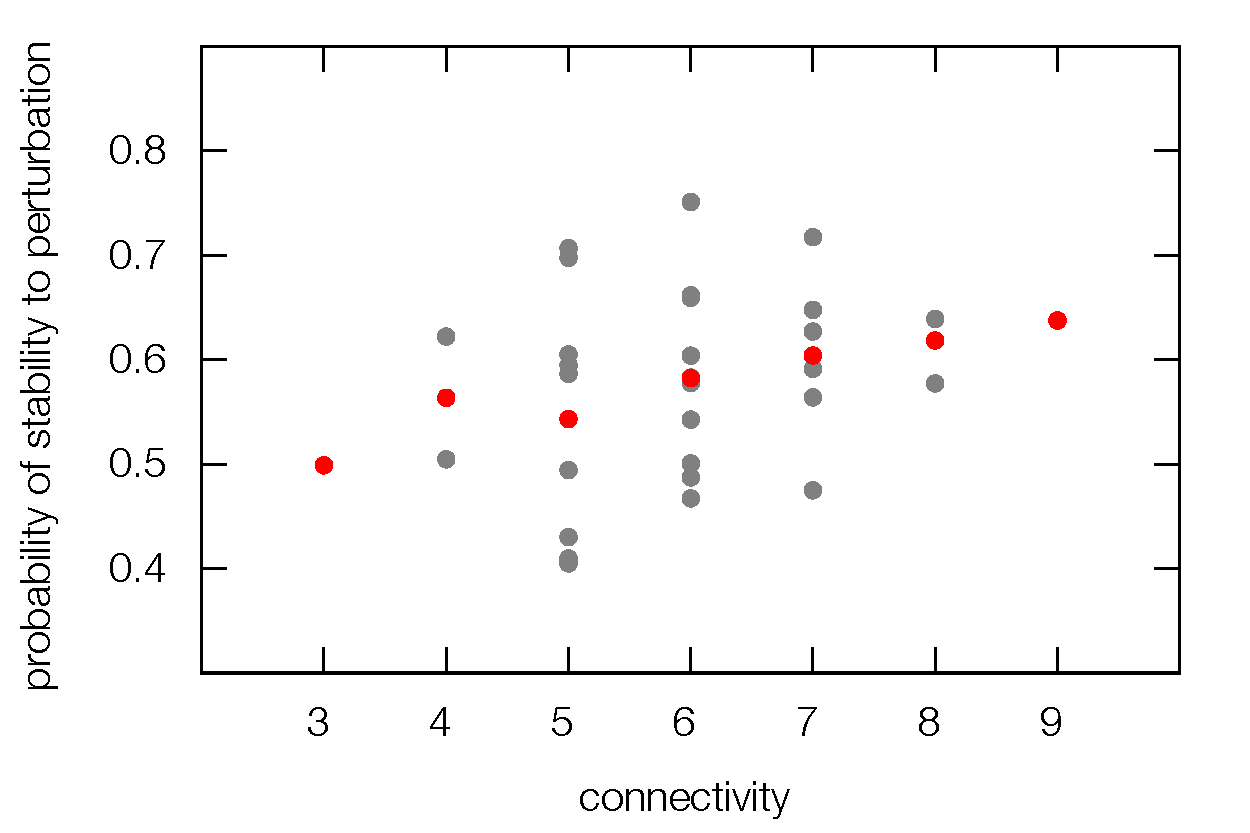
\includegraphics[width=0.8\columnwidth]{fig/stab3x3.pdf}
\caption{{\bf Plot of stability to perturbations versus connectivity for three component systems.} }
\label{fig:stab3x3}
\end{figure}

\begin{figure}[!ht]
\centering
\noindent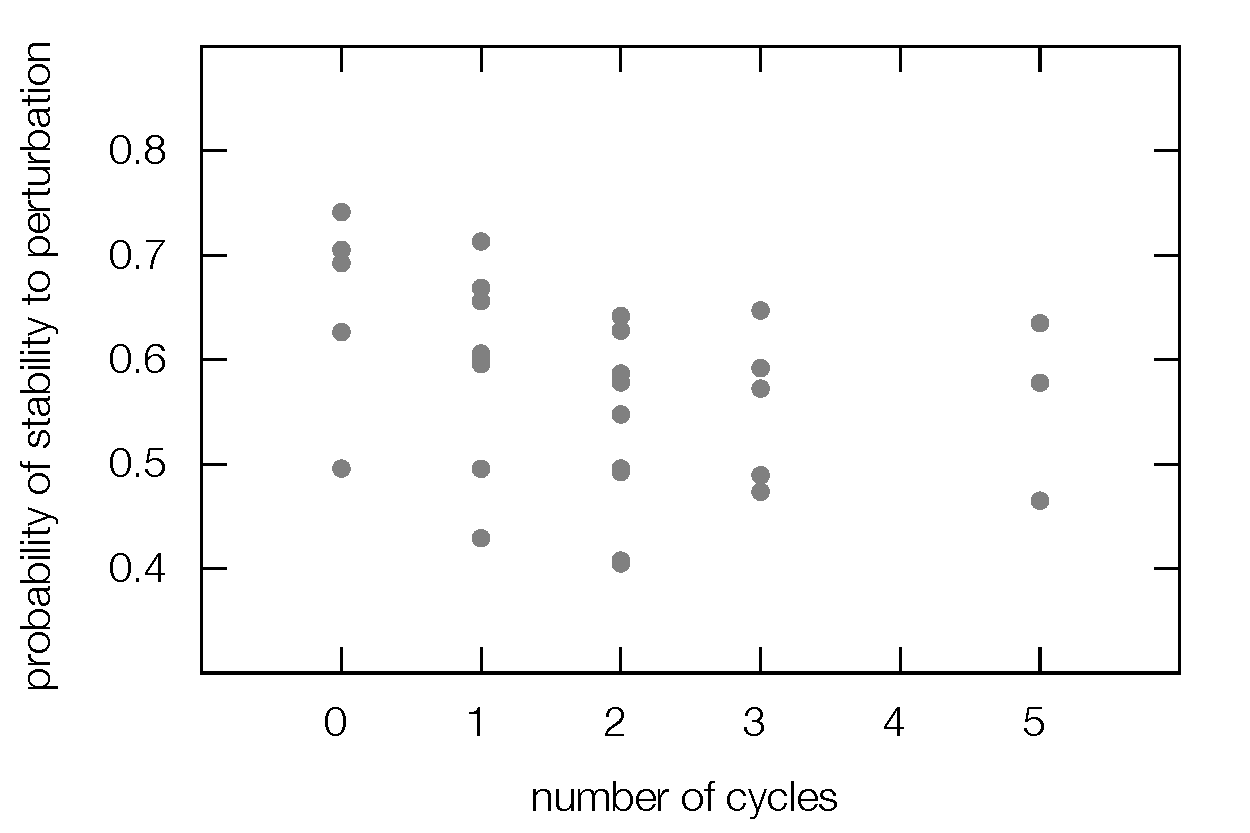
\includegraphics[width=0.8\columnwidth]{fig/cycle3x3.pdf}
\caption{{\bf Plot of stability to perturbations versus number of cycles for three component systems.} }
\label{fig:cycle3x3}
\end{figure}

\pagebreak

% \begin{table}[h]
\begin{longtable}{ c || c | c | c | c }
\hline
matrix & connectivity & cycle number & \specialcell{probability of stability\\to perturbation} & probability of stability\\
\hline
$\begin{pmatrix}
1 & 0 & 0\\
0 & 1 & 0\\
0 & 0 & 1\\
\end{pmatrix}$ & 3 & 0 & 0.496 & 0.122\\
$\begin{pmatrix}
0 & 0 & 1\\
0 & 1 & 0\\
1 & 0 & 1\\
\end{pmatrix}$ & 4 & 1 & 0.496 & 0.13\\
$\begin{pmatrix}
1 & 0 & 0\\
0 & 1 & 1\\
0 & 0 & 1\\
\end{pmatrix}$ & 4 & 0 & 0.626 & 0.128\\
$\begin{pmatrix}
0 & 0 & 1\\
0 & 1 & 1\\
1 & 0 & 1\\
\end{pmatrix}$ & 5 & 1 & 0.602 & 0.127\\
$\begin{pmatrix}
0 & 0 & 1\\
0 & 1 & 1\\
1 & 1 & 0\\
\end{pmatrix}$ & 5 & 2 & 0.496 & 0.122\\
$\begin{pmatrix}
0 & 1 & 1\\
0 & 0 & 1\\
1 & 0 & 1\\
\end{pmatrix}$ & 5 & 2 & 0.405 & 0.061\\
$\begin{pmatrix}
0 & 1 & 0\\
0 & 1 & 1\\
1 & 0 & 1\\
\end{pmatrix}$ & 5 & 1 & 0.429 & 0.081\\
$\begin{pmatrix}
0 & 1 & 1\\
0 & 1 & 0\\
1 & 0 & 1\\
\end{pmatrix}$ & 5 & 1 & 0.597 & 0.129\\
$\begin{pmatrix}
0 & 1 & 1\\
0 & 1 & 1\\
1 & 0 & 0\\
\end{pmatrix}$ & 5 & 2 & 0.408 & 0.062\\
$\begin{pmatrix}
1 & 0 & 1\\
0 & 1 & 1\\
0 & 0 & 1\\
\end{pmatrix}$ & 5 & 0 & 0.693 & 0.125\\
$\begin{pmatrix}
1 & 0 & 0\\
0 & 1 & 1\\
0 & 1 & 1\\
\end{pmatrix}$ & 5 & 1 & 0.606 & 0.124\\
$\begin{pmatrix}
1 & 0 & 1\\
0 & 1 & 0\\
0 & 1 & 1\\
\end{pmatrix}$ & 5 & 0 & 0.705 & 0.131\\
$\begin{pmatrix}
0 & 0 & 1\\
0 & 1 & 1\\
1 & 1 & 1\\
\end{pmatrix}$ & 6 & 2 & 0.578 & 0.115\\
$\begin{pmatrix}
0 & 1 & 1\\
0 & 0 & 1\\
1 & 1 & 1\\
\end{pmatrix}$ & 6 & 3 & 0.489 & 0.085\\
$\begin{pmatrix}
0 & 1 & 1\\
0 & 1 & 1\\
1 & 0 & 1\\
\end{pmatrix}$ & 6 & 2 & 0.548 & 0.091\\
$\begin{pmatrix}
0 & 1 & 0\\
0 & 1 & 1\\
1 & 1 & 1\\
\end{pmatrix}$ & 6 & 2 & 0.493 & 0.087\\
$\begin{pmatrix}
0 & 1 & 1\\
0 & 1 & 0\\
1 & 1 & 1\\
\end{pmatrix}$ & 6 & 1 & 0.669 & 0.128\\
$\begin{pmatrix}
0 & 1 & 1\\
0 & 1 & 1\\
1 & 1 & 0\\
\end{pmatrix}$ & 6 & 3 & 0.474 & 0.086\\
$\begin{pmatrix}
0 & 1 & 1\\
1 & 1 & 0\\
1 & 0 & 1\\
\end{pmatrix}$ & 6 & 2 & 0.587 & 0.12\\
$\begin{pmatrix}
1 & 0 & 1\\
0 & 1 & 1\\
0 & 1 & 1\\
\end{pmatrix}$ & 6 & 1 & 0.656 & 0.121\\
$\begin{pmatrix}
1 & 1 & 1\\
0 & 1 & 1\\
0 & 0 & 1\\
\end{pmatrix}$ & 6 & 0 & 0.741 & 0.125\\
$\begin{pmatrix}
1 & 1 & 0\\
0 & 1 & 1\\
1 & 0 & 1\\
\end{pmatrix}$ & 6 & 1 & 0.596 & 0.098\\
$\begin{pmatrix}
0 & 1 & 1\\
0 & 1 & 1\\
1 & 1 & 1\\
\end{pmatrix}$ & 7 & 3 & 0.572 & 0.094\\
$\begin{pmatrix}
0 & 1 & 1\\
1 & 0 & 1\\
1 & 1 & 1\\
\end{pmatrix}$ & 7 & 5 & 0.465 & 0.075\\
$\begin{pmatrix}
0 & 1 & 1\\
1 & 1 & 1\\
1 & 0 & 1\\
\end{pmatrix}$ & 7 & 3 & 0.592 & 0.105\\
$\begin{pmatrix}
1 & 1 & 1\\
0 & 1 & 1\\
0 & 1 & 1\\
\end{pmatrix}$ & 7 & 1 & 0.713 & 0.122\\
$\begin{pmatrix}
1 & 0 & 1\\
0 & 1 & 1\\
1 & 1 & 1\\
\end{pmatrix}$ & 7 & 2 & 0.642 & 0.125\\
$\begin{pmatrix}
1 & 1 & 1\\
0 & 1 & 1\\
1 & 0 & 1\\
\end{pmatrix}$ & 7 & 2 & 0.628 & 0.11\\
$\begin{pmatrix}
0 & 1 & 1\\
1 & 1 & 1\\
1 & 1 & 1\\
\end{pmatrix}$ & 8 & 5 & 0.578 & 0.092\\
$\begin{pmatrix}
1 & 1 & 1\\
0 & 1 & 1\\
1 & 1 & 1\\
\end{pmatrix}$ & 8 & 3 & 0.647 & 0.115\\
$\begin{pmatrix}
1 & 1 & 1\\
1 & 1 & 1\\
1 & 1 & 1\\
\end{pmatrix}$ & 9 & 5 & 0.635 & 0.11\\
\caption{{\bf Probability of stability under resampling and \emph{a priori} stability for three component systems estimated via Monte Carlo sampling.} All matrices not listed have $0$ probability of stability.}\label{tab:structstabmat3}
\end{longtable}
%
% \end{table}

%!TEX root = ../paper.tex
\begin{longtable}{ c || c | c | c | c }
\hline
matrix & connectivity & cycle number & \specialcell{probability of stability\\to perturbation} & probability of stability\\
\hline
\begin{tikzpicture}[scale=0.6,
every state/.style={draw=red!50,very thick,fill=red!20}]
\begin{dot2tex}[styleonly,codeonly,neato,mathmode]
digraph G {
d2ttikzedgelabels = true;
node [style="state"];
edge [lblstyle="auto",topath="bend left",style="line width=1.5pt"];
1 -> 1 [topath="loop above"];
2 -> 2 [topath="loop above"];
3 -> 3 [topath="loop above"];
}
\end{dot2tex}
\end{tikzpicture} & 3 & 0 & 0.499 & 0.126\\
\begin{tikzpicture}[scale=0.6,
every state/.style={draw=red!50,very thick,fill=red!20}]
\begin{dot2tex}[styleonly,codeonly,neato,mathmode]
digraph G {
d2ttikzedgelabels = true;
node [style="state"];
edge [lblstyle="auto",topath="bend left",style="line width=1.5pt"];
3 -> 1;
2 -> 2 [topath="loop above"];
1 -> 3;
3 -> 3 [topath="loop above"];
}
\end{dot2tex}
\end{tikzpicture} & 4 & 1 & 0.505 & 0.121\\
\begin{tikzpicture}[scale=0.6,
every state/.style={draw=red!50,very thick,fill=red!20}]
\begin{dot2tex}[styleonly,codeonly,neato,mathmode]
digraph G {
d2ttikzedgelabels = true;
node [style="state"];
edge [lblstyle="auto",topath="bend left",style="line width=1.5pt"];
1 -> 1 [topath="loop above"];
2 -> 2 [topath="loop above"];
3 -> 2;
3 -> 3 [topath="loop above"];
}
\end{dot2tex}
\end{tikzpicture} & 4 & 0 & 0.622 & 0.127\\
\begin{tikzpicture}[scale=0.6,
every state/.style={draw=red!50,very thick,fill=red!20}]
\begin{dot2tex}[styleonly,codeonly,neato,mathmode]
digraph G {
d2ttikzedgelabels = true;
node [style="state"];
edge [lblstyle="auto",topath="bend left",style="line width=1.5pt"];
3 -> 1;
2 -> 2 [topath="loop above"];
3 -> 2;
1 -> 3;
3 -> 3 [topath="loop above"];
}
\end{dot2tex}
\end{tikzpicture} & 5 & 1 & 0.595 & 0.121\\
\begin{tikzpicture}[scale=0.6,
every state/.style={draw=red!50,very thick,fill=red!20}]
\begin{dot2tex}[styleonly,codeonly,neato,mathmode]
digraph G {
d2ttikzedgelabels = true;
node [style="state"];
edge [lblstyle="auto",topath="bend left",style="line width=1.5pt"];
3 -> 1;
2 -> 2 [topath="loop above"];
3 -> 2;
1 -> 3;
2 -> 3;
}
\end{dot2tex}
\end{tikzpicture} & 5 & 2 & 0.494 & 0.128\\
\begin{tikzpicture}[scale=0.6,
every state/.style={draw=red!50,very thick,fill=red!20}]
\begin{dot2tex}[styleonly,codeonly,neato,mathmode]
digraph G {
d2ttikzedgelabels = true;
node [style="state"];
edge [lblstyle="auto",topath="bend left",style="line width=1.5pt"];
2 -> 1;
3 -> 1;
3 -> 2;
1 -> 3;
3 -> 3 [topath="loop above"];
}
\end{dot2tex}
\end{tikzpicture} & 5 & 2 & 0.41 & 0.061\\
\begin{tikzpicture}[scale=0.6,
every state/.style={draw=red!50,very thick,fill=red!20}]
\begin{dot2tex}[styleonly,codeonly,neato,mathmode]
digraph G {
d2ttikzedgelabels = true;
node [style="state"];
edge [lblstyle="auto",topath="bend left",style="line width=1.5pt"];
2 -> 1;
2 -> 2 [topath="loop above"];
3 -> 2;
1 -> 3;
3 -> 3 [topath="loop above"];
}
\end{dot2tex}
\end{tikzpicture} & 5 & 1 & 0.43 & 0.078\\
\begin{tikzpicture}[scale=0.6,
every state/.style={draw=red!50,very thick,fill=red!20}]
\begin{dot2tex}[styleonly,codeonly,neato,mathmode]
digraph G {
d2ttikzedgelabels = true;
node [style="state"];
edge [lblstyle="auto",topath="bend left",style="line width=1.5pt"];
2 -> 1;
3 -> 1;
2 -> 2 [topath="loop above"];
1 -> 3;
3 -> 3 [topath="loop above"];
}
\end{dot2tex}
\end{tikzpicture} & 5 & 1 & 0.605 & 0.12\\
\begin{tikzpicture}[scale=0.6,
every state/.style={draw=red!50,very thick,fill=red!20}]
\begin{dot2tex}[styleonly,codeonly,neato,mathmode]
digraph G {
d2ttikzedgelabels = true;
node [style="state"];
edge [lblstyle="auto",topath="bend left",style="line width=1.5pt"];
2 -> 1;
3 -> 1;
2 -> 2 [topath="loop above"];
3 -> 2;
1 -> 3;
}
\end{dot2tex}
\end{tikzpicture} & 5 & 2 & 0.405 & 0.06\\
\begin{tikzpicture}[scale=0.6,
every state/.style={draw=red!50,very thick,fill=red!20}]
\begin{dot2tex}[styleonly,codeonly,neato,mathmode]
digraph G {
d2ttikzedgelabels = true;
node [style="state"];
edge [lblstyle="auto",topath="bend left",style="line width=1.5pt"];
1 -> 1 [topath="loop above"];
3 -> 1;
2 -> 2 [topath="loop above"];
3 -> 2;
3 -> 3 [topath="loop above"];
}
\end{dot2tex}
\end{tikzpicture} & 5 & 0 & 0.698 & 0.122\\
\begin{tikzpicture}[scale=0.6,
every state/.style={draw=red!50,very thick,fill=red!20}]
\begin{dot2tex}[styleonly,codeonly,neato,mathmode]
digraph G {
d2ttikzedgelabels = true;
node [style="state"];
edge [lblstyle="auto",topath="bend left",style="line width=1.5pt"];
1 -> 1 [topath="loop above"];
2 -> 2 [topath="loop above"];
3 -> 2;
2 -> 3;
3 -> 3 [topath="loop above"];
}
\end{dot2tex}
\end{tikzpicture} & 5 & 1 & 0.587 & 0.128\\
\begin{tikzpicture}[scale=0.6,
every state/.style={draw=red!50,very thick,fill=red!20}]
\begin{dot2tex}[styleonly,codeonly,neato,mathmode]
digraph G {
d2ttikzedgelabels = true;
node [style="state"];
edge [lblstyle="auto",topath="bend left",style="line width=1.5pt"];
1 -> 1 [topath="loop above"];
3 -> 1;
2 -> 2 [topath="loop above"];
2 -> 3;
3 -> 3 [topath="loop above"];
}
\end{dot2tex}
\end{tikzpicture} & 5 & 0 & 0.707 & 0.127\\
\begin{tikzpicture}[scale=0.6,
every state/.style={draw=red!50,very thick,fill=red!20}]
\begin{dot2tex}[styleonly,codeonly,neato,mathmode]
digraph G {
d2ttikzedgelabels = true;
node [style="state"];
edge [lblstyle="auto",topath="bend left",style="line width=1.5pt"];
3 -> 1;
2 -> 2 [topath="loop above"];
3 -> 2;
1 -> 3;
2 -> 3;
3 -> 3 [topath="loop above"];
}
\end{dot2tex}
\end{tikzpicture} & 6 & 2 & 0.578 & 0.121\\
\begin{tikzpicture}[scale=0.6,
every state/.style={draw=red!50,very thick,fill=red!20}]
\begin{dot2tex}[styleonly,codeonly,neato,mathmode]
digraph G {
d2ttikzedgelabels = true;
node [style="state"];
edge [lblstyle="auto",topath="bend left",style="line width=1.5pt"];
2 -> 1;
3 -> 1;
3 -> 2;
1 -> 3;
2 -> 3;
3 -> 3 [topath="loop above"];
}
\end{dot2tex}
\end{tikzpicture} & 6 & 3 & 0.487 & 0.081\\
\begin{tikzpicture}[scale=0.6,
every state/.style={draw=red!50,very thick,fill=red!20}]
\begin{dot2tex}[styleonly,codeonly,neato,mathmode]
digraph G {
d2ttikzedgelabels = true;
node [style="state"];
edge [lblstyle="auto",topath="bend left",style="line width=1.5pt"];
2 -> 1;
3 -> 1;
2 -> 2 [topath="loop above"];
3 -> 2;
1 -> 3;
3 -> 3 [topath="loop above"];
}
\end{dot2tex}
\end{tikzpicture} & 6 & 2 & 0.543 & 0.098\\
\begin{tikzpicture}[scale=0.6,
every state/.style={draw=red!50,very thick,fill=red!20}]
\begin{dot2tex}[styleonly,codeonly,neato,mathmode]
digraph G {
d2ttikzedgelabels = true;
node [style="state"];
edge [lblstyle="auto",topath="bend left",style="line width=1.5pt"];
2 -> 1;
2 -> 2 [topath="loop above"];
3 -> 2;
1 -> 3;
2 -> 3;
3 -> 3 [topath="loop above"];
}
\end{dot2tex}
\end{tikzpicture} & 6 & 2 & 0.501 & 0.088\\
\begin{tikzpicture}[scale=0.6,
every state/.style={draw=red!50,very thick,fill=red!20}]
\begin{dot2tex}[styleonly,codeonly,neato,mathmode]
digraph G {
d2ttikzedgelabels = true;
node [style="state"];
edge [lblstyle="auto",topath="bend left",style="line width=1.5pt"];
2 -> 1;
3 -> 1;
2 -> 2 [topath="loop above"];
1 -> 3;
2 -> 3;
3 -> 3 [topath="loop above"];
}
\end{dot2tex}
\end{tikzpicture} & 6 & 1 & 0.662 & 0.123\\
\begin{tikzpicture}[scale=0.6,
every state/.style={draw=red!50,very thick,fill=red!20}]
\begin{dot2tex}[styleonly,codeonly,neato,mathmode]
digraph G {
d2ttikzedgelabels = true;
node [style="state"];
edge [lblstyle="auto",topath="bend left",style="line width=1.5pt"];
2 -> 1;
3 -> 1;
2 -> 2 [topath="loop above"];
3 -> 2;
1 -> 3;
2 -> 3;
}
\end{dot2tex}
\end{tikzpicture} & 6 & 3 & 0.467 & 0.079\\
\begin{tikzpicture}[scale=0.6,
every state/.style={draw=red!50,very thick,fill=red!20}]
\begin{dot2tex}[styleonly,codeonly,neato,mathmode]
digraph G {
d2ttikzedgelabels = true;
node [style="state"];
edge [lblstyle="auto",topath="bend left",style="line width=1.5pt"];
2 -> 1;
3 -> 1;
1 -> 2;
2 -> 2 [topath="loop above"];
1 -> 3;
3 -> 3 [topath="loop above"];
}
\end{dot2tex}
\end{tikzpicture} & 6 & 2 & 0.583 & 0.13\\
\begin{tikzpicture}[scale=0.6,
every state/.style={draw=red!50,very thick,fill=red!20}]
\begin{dot2tex}[styleonly,codeonly,neato,mathmode]
digraph G {
d2ttikzedgelabels = true;
node [style="state"];
edge [lblstyle="auto",topath="bend left",style="line width=1.5pt"];
1 -> 1 [topath="loop above"];
3 -> 1;
2 -> 2 [topath="loop above"];
3 -> 2;
2 -> 3;
3 -> 3 [topath="loop above"];
}
\end{dot2tex}
\end{tikzpicture} & 6 & 1 & 0.659 & 0.124\\
\begin{tikzpicture}[scale=0.6,
every state/.style={draw=red!50,very thick,fill=red!20}]
\begin{dot2tex}[styleonly,codeonly,neato,mathmode]
digraph G {
d2ttikzedgelabels = true;
node [style="state"];
edge [lblstyle="auto",topath="bend left",style="line width=1.5pt"];
1 -> 1 [topath="loop above"];
2 -> 1;
3 -> 1;
2 -> 2 [topath="loop above"];
3 -> 2;
3 -> 3 [topath="loop above"];
}
\end{dot2tex}
\end{tikzpicture} & 6 & 0 & 0.751 & 0.124\\
\begin{tikzpicture}[scale=0.6,
every state/.style={draw=red!50,very thick,fill=red!20}]
\begin{dot2tex}[styleonly,codeonly,neato,mathmode]
digraph G {
d2ttikzedgelabels = true;
node [style="state"];
edge [lblstyle="auto",topath="bend left",style="line width=1.5pt"];
1 -> 1 [topath="loop above"];
2 -> 1;
2 -> 2 [topath="loop above"];
3 -> 2;
1 -> 3;
3 -> 3 [topath="loop above"];
}
\end{dot2tex}
\end{tikzpicture} & 6 & 1 & 0.604 & 0.097\\
\begin{tikzpicture}[scale=0.6,
every state/.style={draw=red!50,very thick,fill=red!20}]
\begin{dot2tex}[styleonly,codeonly,neato,mathmode]
digraph G {
d2ttikzedgelabels = true;
node [style="state"];
edge [lblstyle="auto",topath="bend left",style="line width=1.5pt"];
2 -> 1;
3 -> 1;
2 -> 2 [topath="loop above"];
3 -> 2;
1 -> 3;
2 -> 3;
3 -> 3 [topath="loop above"];
}
\end{dot2tex}
\end{tikzpicture} & 7 & 3 & 0.564 & 0.103\\
\begin{tikzpicture}[scale=0.6,
every state/.style={draw=red!50,very thick,fill=red!20}]
\begin{dot2tex}[styleonly,codeonly,neato,mathmode]
digraph G {
d2ttikzedgelabels = true;
node [style="state"];
edge [lblstyle="auto",topath="bend left",style="line width=1.5pt"];
2 -> 1;
3 -> 1;
1 -> 2;
3 -> 2;
1 -> 3;
2 -> 3;
3 -> 3 [topath="loop above"];
}
\end{dot2tex}
\end{tikzpicture} & 7 & 5 & 0.475 & 0.068\\
\begin{tikzpicture}[scale=0.6,
every state/.style={draw=red!50,very thick,fill=red!20}]
\begin{dot2tex}[styleonly,codeonly,neato,mathmode]
digraph G {
d2ttikzedgelabels = true;
node [style="state"];
edge [lblstyle="auto",topath="bend left",style="line width=1.5pt"];
2 -> 1;
3 -> 1;
1 -> 2;
2 -> 2 [topath="loop above"];
3 -> 2;
1 -> 3;
3 -> 3 [topath="loop above"];
}
\end{dot2tex}
\end{tikzpicture} & 7 & 3 & 0.591 & 0.108\\
\begin{tikzpicture}[scale=0.6,
every state/.style={draw=red!50,very thick,fill=red!20}]
\begin{dot2tex}[styleonly,codeonly,neato,mathmode]
digraph G {
d2ttikzedgelabels = true;
node [style="state"];
edge [lblstyle="auto",topath="bend left",style="line width=1.5pt"];
1 -> 1 [topath="loop above"];
2 -> 1;
3 -> 1;
2 -> 2 [topath="loop above"];
3 -> 2;
2 -> 3;
3 -> 3 [topath="loop above"];
}
\end{dot2tex}
\end{tikzpicture} & 7 & 1 & 0.717 & 0.119\\
\begin{tikzpicture}[scale=0.6,
every state/.style={draw=red!50,very thick,fill=red!20}]
\begin{dot2tex}[styleonly,codeonly,neato,mathmode]
digraph G {
d2ttikzedgelabels = true;
node [style="state"];
edge [lblstyle="auto",topath="bend left",style="line width=1.5pt"];
1 -> 1 [topath="loop above"];
3 -> 1;
2 -> 2 [topath="loop above"];
3 -> 2;
1 -> 3;
2 -> 3;
3 -> 3 [topath="loop above"];
}
\end{dot2tex}
\end{tikzpicture} & 7 & 2 & 0.648 & 0.122\\
\begin{tikzpicture}[scale=0.6,
every state/.style={draw=red!50,very thick,fill=red!20}]
\begin{dot2tex}[styleonly,codeonly,neato,mathmode]
digraph G {
d2ttikzedgelabels = true;
node [style="state"];
edge [lblstyle="auto",topath="bend left",style="line width=1.5pt"];
1 -> 1 [topath="loop above"];
2 -> 1;
3 -> 1;
2 -> 2 [topath="loop above"];
3 -> 2;
1 -> 3;
3 -> 3 [topath="loop above"];
}
\end{dot2tex}
\end{tikzpicture} & 7 & 2 & 0.627 & 0.105\\
\begin{tikzpicture}[scale=0.6,
every state/.style={draw=red!50,very thick,fill=red!20}]
\begin{dot2tex}[styleonly,codeonly,neato,mathmode]
digraph G {
d2ttikzedgelabels = true;
node [style="state"];
edge [lblstyle="auto",topath="bend left",style="line width=1.5pt"];
2 -> 1;
3 -> 1;
1 -> 2;
2 -> 2 [topath="loop above"];
3 -> 2;
1 -> 3;
2 -> 3;
3 -> 3 [topath="loop above"];
}
\end{dot2tex}
\end{tikzpicture} & 8 & 5 & 0.577 & 0.093\\
\begin{tikzpicture}[scale=0.6,
every state/.style={draw=red!50,very thick,fill=red!20}]
\begin{dot2tex}[styleonly,codeonly,neato,mathmode]
digraph G {
d2ttikzedgelabels = true;
node [style="state"];
edge [lblstyle="auto",topath="bend left",style="line width=1.5pt"];
1 -> 1 [topath="loop above"];
2 -> 1;
3 -> 1;
2 -> 2 [topath="loop above"];
3 -> 2;
1 -> 3;
2 -> 3;
3 -> 3 [topath="loop above"];
}
\end{dot2tex}
\end{tikzpicture} & 8 & 3 & 0.639 & 0.109\\
\begin{tikzpicture}[scale=0.6,
every state/.style={draw=red!50,very thick,fill=red!20}]
\begin{dot2tex}[styleonly,codeonly,neato,mathmode]
digraph G {
d2ttikzedgelabels = true;
node [style="state"];
edge [lblstyle="auto",topath="bend left",style="line width=1.5pt"];
1 -> 1 [topath="loop above"];
2 -> 1;
3 -> 1;
1 -> 2;
2 -> 2 [topath="loop above"];
3 -> 2;
1 -> 3;
2 -> 3;
3 -> 3 [topath="loop above"];
}
\end{dot2tex}
\end{tikzpicture} & 9 & 5 & 0.638 & 0.106\\
\caption{{\bf Probability of stability under resampling and \emph{a priori} stability for three variable systems estimated via Monte Carlo sampling.} All matrices not listed have $0$ probability of stability.}\label{tab:structstabmat3graph}
\end{longtable}


\bibliographystyle{amsplain}
\bibliography{bib/books,bib/papers}

\section{Appendix A}\label{sec:appA}
Suppose that we have a family
of polynomials whose roots are of one type but turn into another type.
There are three ways this could happen:
\begin{itemize}
\item{1.} A real root could go from being positive to being negative
  or vice versa.  For this to happen, we must pass through an
  intermediate value with a zero root.  For that intermediate value,
  we have $D = 0$.
\item{2.} A pair of real roots could turn into a pair of complex roots
  or vice versa.  For this to happen, we must pass through an
  intermediate value with a repeated root.  For that intermediate
  value, we have $\delta = 0$.
\item{3.} A conjugate pair of complex roots could go from having
  positive real part to having negative real part or vice versa.  For
  this to happen, we must pass through an intermediate value in which
  the real part is zero.  For that intermediate value, the two roots
  are imaginary so, bing conjugates, they sum to zero, hence we have
  $\Delta = 0$.
\end{itemize}
\noindent  Thus, we conclude that the boundaries of our regions
$R_{abcd}$ consist of portions of the surfaces $D=0, \delta=0,
\Delta=0$ and we will characterize them by studying these surfaces.

\end{document}

%------------------------------------------------------------------------------
% End of journal.tex
%------------------------------------------------------------------------------
